% !TEX root = handbook-physics.tex
%!TEX TS-program = pdflatex
%!TEX encoding = UTF-8 Unicode






\chapter{Capacitance}
\label{ch-17}
\zhtitle{电容}

\section{Capacitance of an Isolated Conductor}
\label{sec-17.1}
\zhtitle{孤立导体的电容}

\subsection{}\label{17.1.1} Upon an increase in the amount of electricity transmitted to an isolated conductor, the charges are distributed over the conductor's surface with varying surface density. The way in which the charges are distributed depends only on the shape of the conductor, but not on the amount of electricity that was previously on the conductor. Each new portion of charges is distributed over the surface of the conductor similar to the preceding portion. It follows that, at any point on the conductor's surface, the surface charge density $\sigma$ \ssect{15.2.3} increases in proportion to the charge $q$ on the conductor: $\sigma = kq$, where $k = f \,(x, \,y,\, z)$ is a function of the coordinates of the point being considered on the surface.
\zhpar{当传递给孤立导体的电量增加时，电荷以不同的面密度分布在导体表面上。电荷的分布方式仅取决于导体的形状，而与导体上原有的电量无关。每一部分新增的电荷都以与前一部分相似的方式分布在导体表面上。由此可知，导体表面上任一点的面电荷密度 $\sigma$ \ssect{15.2.3} 与导体所带电荷 $q$ 成正比增大：$\sigma = kq$，其中 $k = f \,(x, \,y,\, z)$ 是所考察的表面点坐标的函数。}

The potential of the field set up by a charged conductor \ssect{16.2.6} is
\zhpar{带电导体所建立场的电势（\ssect{16.2.6}）为：}
\begin{equation*}%
V =\frac{1}{4 \pi \varepsilon_{0}\varepsilon_{r}} \oint_{S} \frac{\sigma \, \dd S}{r} = \frac{q}{4 \pi \varepsilon_{0}\varepsilon_{r}} =  \oint_{S} \frac{k \, \dd S}{r}.
\end{equation*}
For points on the surface $S$ of the conductor this integral depends only on the size and shape of the conductor's surface. Hence the potential $V$ of the conductor is proportional to its charge $q$.
\zhpar{对于导体表面 $S$ 上的点，该积分仅取决于导体表面的大小和形状。因此，导体的电势 $V$ 与其所带电荷 $q$ 成正比。}

\subsection{}\label{17.1.2}The ratio of the charge $q$ of an isolated conductor to its potential $V$ is called the \redem{capacitance} of the given conductor:
\zhpar{孤立导体所带电荷 $q$ 与其电势 $V$ 之比，称为该导体的\redem{电容}：}
\begin{align*}
C & = \frac{q}{V} && \text{or} \\
C & = \fpee \left( \oint_{S} \frac{k \, \dd S}{r} \right)^{-1} && \text{(in SI units.)}
\end{align*}
The capacitance of an isolated conductor is numerically equal to the charge that changes the potential of the conductor by one unit.
\zhpar{孤立导体的电容在数值上等于使导体电势改变一个单位所需的电荷量。}

The capacitance of an isolated conductor depends upon its shape and dimensions. For geometrically similar conductors, their capacitances are proportional to their linear dimen­sions.
\zhpar{孤立导体的电容取决于其形状和尺寸。对于几何相似的导体，其电容与线性尺寸成正比。}

The capacitance of an isolated conductor depends upon the dielectric properties of the surrounding medium. The capacitance of a conductor in a homogeneous isotropic medium is proportional to the relative permittivity (dielectric constant) \ssect{14.2.4} of the medium.
\zhpar{孤立导体的电容还取决于周围介质的介电性质。在均匀各向同性介质中，导体的电容与介质的相对电容率（又称相对介电常量）成正比（\ssect{14.2.4}）。}

\subsection{}\label{17.1.3} It follows from the equation for the potential of an isolated conducting sphere of radius $R$ \ssect{16.2.6} that the \redem{capacitance} of such a \redem{sphere} is
\zhpar{由半径为 $R$ 的孤立导体球的电势方程（\ssect{16.2.6}）可知，这种\redem{球体}的\redem{电容}为：}
\begin{align*}
C & = \fpee \, R && \text{(in SI units.)} \\
C & = \varepsilon_{r}\,R && \text{(in cgse units.)}
\end{align*}




\section{Mutual Capacitance. Capacitors}
\label{sec-17.2}
\zhtitle{互电容。电容器}

\subsection{}\label{17.2.1} When there are other conductors close to conductor $A$ the capacitance of the latter is greater than for an identical, but isolated, conductor. This is due to the fact that when the charge $q$ is transferred to conductor $A$,charges are induced on the conductors surrounding it under the influence of the field set up by conductor $A$. The portions of the surrounding conductors nearest to the inducing charge $q$ become oppositely charged (\figr{fig-17-01}). These charges weaken the field set up by charge $q$ lower the potential of conductor $A$ and increase its capacitance.
\zhpar{当导体 $A$ 附近存在其他导体时，导体 $A$ 的电容大于形状相同但孤立的导体的电容。这是因为，当电荷 $q$ 传给导体 $A$ 时，在导体 $A$ 所建立场的作用下，周围的导体上会感应出电荷。离感应电荷 $q$ 最近的那部分周围导体带上异号电荷（\figr{fig-17-01}）。这些电荷削弱了电荷 $q$ 所建立的场，降低了导体 $A$ 的电势，从而增大了其电容。}

\begin{marginfigure}
\centering
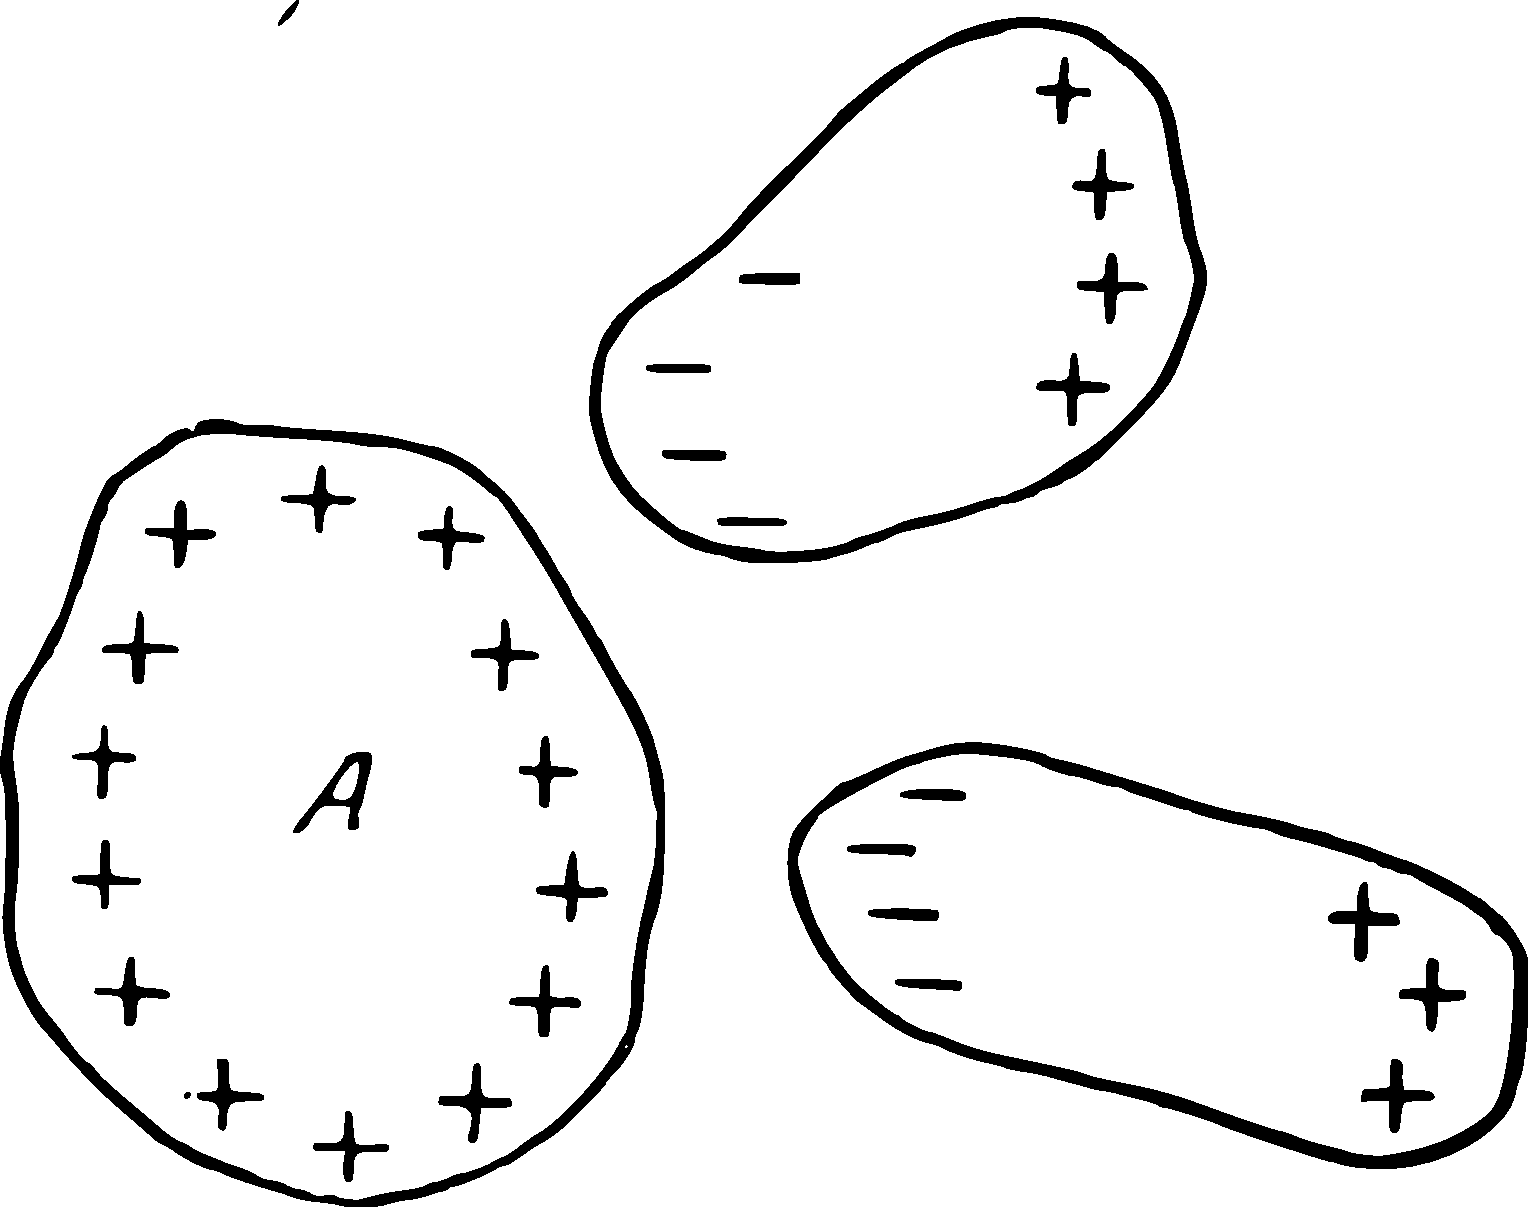
\includegraphics[width=\textwidth]{figs/ch-17/fig-17-01.pdf}
\caption{Induced charges in conductors.\zhcap{导体中的感应电荷。}\label{fig-17-01}}
\end{marginfigure}
\subsection{}\label{17.2.2} In a system of two conductors arranged close to each
oilier, having charges $q$ equal in magnitude but opposite in sign, a potential difference $V_{1} - V_{2}$ is produced that is proportional to $q$:
\zhpar{在两个靠近放置、所带电荷数值相等而符号相反的导体所构成的系统中，两导体间产生的电势差 $V_{1} - V_{2}$ 与 $q$ 成正比：}
\begin{equation*}%
V_{1} - V_{2} = \frac{1}{C} \, q,
\end{equation*}
where $C = q/(V_{1} - V_{2})$ is the \redem{mutual capacitance} of the two conductors.
\zhpar{式中 $C = q/(V_{1} - V_{2})$ 即两导体的\redem{互电容}。}

The mutual capacitance of two conductors is numerically equal to the charge that it is necessary to transfer from one conductor to the other to change the potential difference between them by one unit.
\zhpar{两导体的互电容在数值上等于将电荷从一个导体转移到另一个导体，使两者之间的电势差改变一个单位所需转移的电荷量。}

\subsection{}\label{17.2.3} The mutual capacitance $C$ of two conductors depends upon their shapes, dimensions and relative positions. Moreover, $C$ depends upon the dielectric properties of the medium surrounding the conductors. If the medium is homogeneous and isotropic, $C$ is directly proportional to the relative permittivity \ssect{14.2.4} of the medium.
\zhpar{两导体的互电容 $C$ 取决于它们的形状、尺寸和相对位置。此外，$C$ 还取决于导体周围介质的介电性质。若介质均匀且各向同性，则 $C$ 与介质的相对电容率（\ssect{14.2.4}）成正比。}

When one of the conductors is moved away to infinity, the potential difference $V_{1} - V_{2}$ between them increases and their mutual capacitance is reduced, tending to the capacitance of the remaining isolated conductor.
\zhpar{当其中一个导体被移到无穷远时，两者间的电势差 $V_{1} - V_{2}$ 增大，互电容减小，并趋于剩余的孤立导体的电容。}

\subsection{}\label{17.2.4} A \redem{capacitor} is a system of two charged conductors, insulated from each other and having charges of equal magnitude and opposite sign, provided that their shapes and relative position are such that the conductors set up a concentrated electrostatic field in a limited region of space. In the case of parallel-plate capacitors, the conductors are called \redem{plates}. The capacitance of a capacitor is the mutual capacitance of its plates (or, in the general case, conductors).
\zhpar{\redem{电容器}是由两个带电导体构成的系统。两导体彼此绝缘，所带电荷数值相等、符号相反，且其形状和相对位置使二者能在有限的空间区域内建立集中的静电场。对于平行板电容器，导体称为\redem{极板}。电容器的电容即其两极板（或一般情形下的两导体）之间的互电容。}




\subsection{}\label{17.2.5} The capacitance of a \redem{parallel-plate capacitor}, consisting of two metal plates, is
\zhpar{由两块金属平板组成的\redem{平行板电容器}，其电容为：}
\begin{align*}
C & = \frac{\varepsilon_{0}\varepsilon_{r}S}{d} && \text{(in SI units.)} \\
C & = \frac{\varepsilon_{r}S}{4 \pi d} && \text{(in cgse units.)}
\end{align*}
where $\varepsilon_{r}$ is the relative permittivity of the medium filling the space between the plates, $S$ is the area of each plate, and $d$ is the distance between them. For a multiple-plate capacitor consisting of $n$ plates, the formula for the capacitance contains $S(n - 1)$ instead of $S$. The capacitance formula is valid only for small d values, when the lack of uniformity of the electrostatic field at the edges of the capacitor plates can be ignored. 
\zhpar{式中 $\varepsilon_{r}$ 为充满两极板之间空间的介质的相对电容率，$S$ 为每块极板的面积，$d$ 为两极板之间的距离。对于由 $n$ 块极板组成的多极板电容器，电容公式中的 $S$ 应换为 $S(n - 1)$。该公式仅在 $d$ 值较小、可忽略极板边缘处静电场的不均匀性时才成立。}


\begin{marginfigure}[-3cm]
\centering
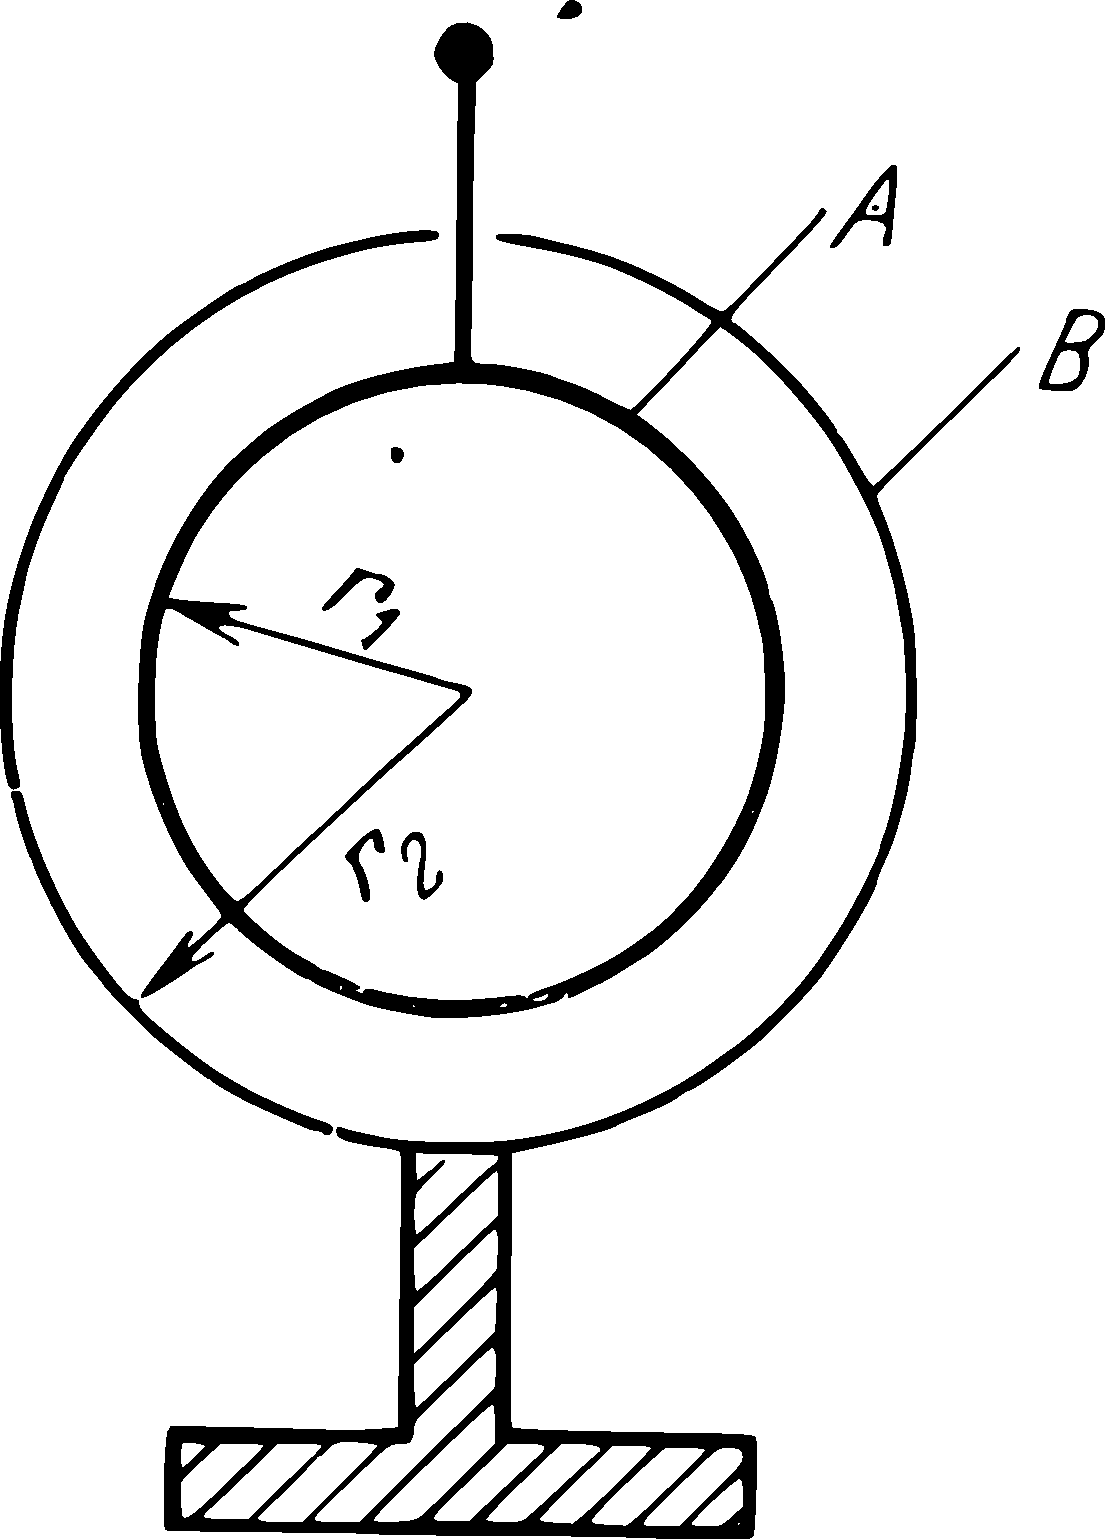
\includegraphics[width=0.8\textwidth]{figs/ch-17/fig-17-02.pdf}
\caption{A spherical capacitor.\zhcap{球形电容器。}\label{fig-17-02}}
\end{marginfigure}
\subsection{}\label{17.2.6} A \redem{spherical capacitor} consists of two concentric hollow metal spheres $A$ and $B$, of radii $r_{1}$ and $r_{2}$ (\figr{fig-17-02}). The spheres are charged on their surfaces and set up fields only outside themselves \ssect{15.1.4}. Hence, in the space between the spheres the field is set up only by the charge of sphere $A$. Outside the capacitor, the fields of the oppositely charged spheres $A$ and $B$ mutually eliminate each other.
\zhpar{\redem{球形电容器}由两个同心的空心金属球 $A$ 和 $B$ 组成，其半径分别为 $r_{1}$ 和 $r_{2}$（见\figr{fig-17-02}）。两球的电荷分布在各自表面上，且只在球外产生场（\ssect{15.1.4}）。因此，在两球之间的空间中，场仅由球 $A$ 的电荷产生。在电容器外部，带异号电荷的球 $A$ 与球 $B$ 的场相互抵消。}


The capacitance of a spherical capacitor is calculated by the formula
\zhpar{球形电容器的电容由下式计算：}
\begin{align*}
C & = \frac{\fpee\, r_{1} r_{2}}{r_{2} - r_{1}} && \text{(in SI units.)} \\
C & = \frac{\varepsilon_{r}\,r_{1} r_{2}}{r_{2} - r_{1}}&& \text{(in cgse units.)}
\end{align*}
As $r_{2} \to \infty$ and $1/r_{2} \to 0$, the inner sphere becomes an isolated one and $C = \fpee \, r_{1}$ (cf. \ssect{17.1.3}). For any finite values of $r_{1}$ and $r_{2}$
\zhpar{当 $r_{2} \to \infty$、$1/r_{2} \to 0$ 时，内球变为孤立球，此时 $C = \fpee \, r_{1}$（参见 \ssect{17.1.3}）。对于 $r_{1}$ 和 $r_{2}$ 的任意有限值，有：}
\begin{equation*}%
C= \fpee \, r_{1} \, \frac{r_{2}}{r_{2} - r_{1}} > \fpee \, r_{1},
\end{equation*}
i.e. the capacitance of a spherical capacitor is greater than that of an isolated hollow sphere.
\zhpar{即球形电容器的电容大于孤立空心球的电容。}


\begin{marginfigure}[-3cm]
\centering
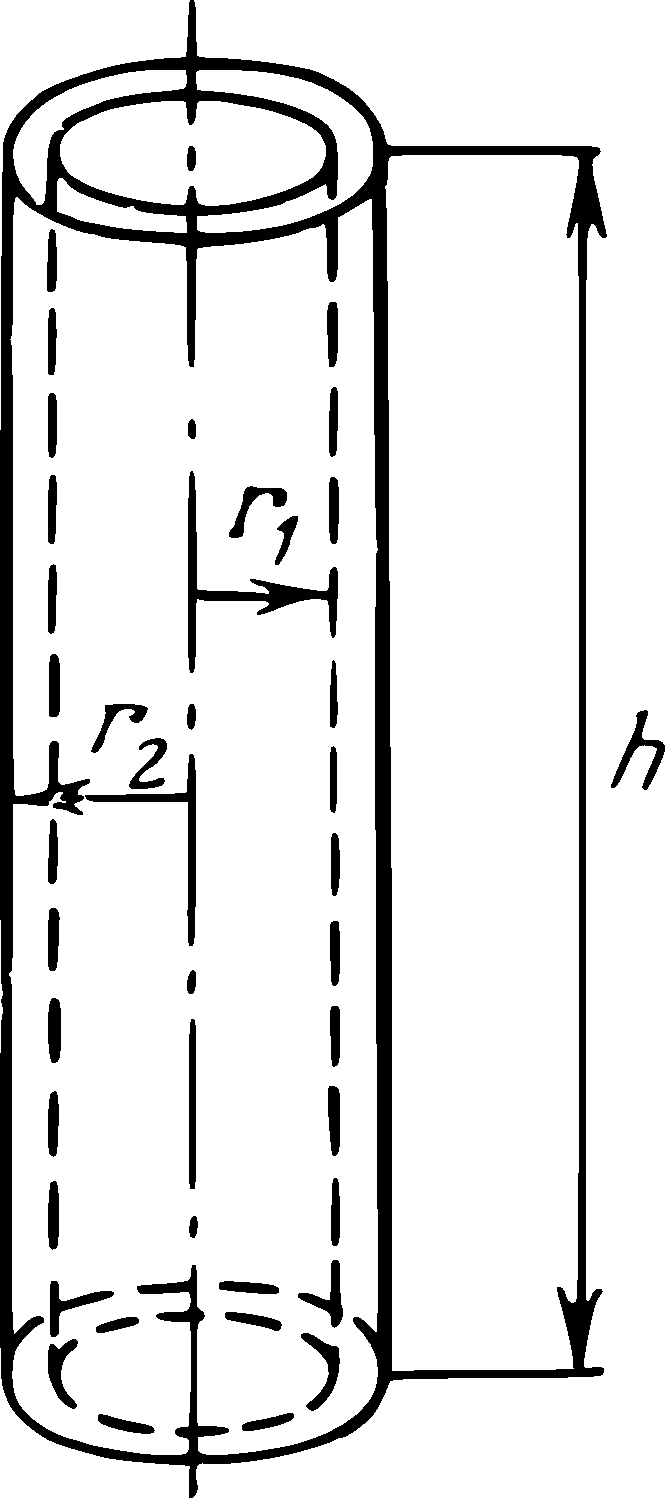
\includegraphics[width=0.5\textwidth]{figs/ch-17/fig-17-03.pdf}
\caption{A cylindrical capacitor.\zhcap{圆柱形电容器。}\label{fig-17-03}}
\end{marginfigure}


\subsection{}\label{17.2.7} A \redem{cylindrical capacitor} consists of two hollow coaxial metal cylinders of height $h$ and radii $r_{1}$ and $r_{2}$ (\figr{fig-17-02}). The formula for the capacitance of a cylindrical capacitor (or of a coaxial cable) is of the form
\zhpar{\redem{圆柱形电容器}由两个同轴的空心金属圆柱组成，其高度为 $h$，半径分别为 $r_{1}$ 和 $r_{2}$（见\figr{fig-17-02}）。圆柱形电容器（或同轴电缆）的电容公式具有如下形式：}
\begin{align*}
C & = \frac{2 \pi \ee h}{\ln r_{2}/r_{1}} && \text{(in SI units.)} \\
C & = \frac{\varepsilon_{r} h}{2 \ln r_{2}/r_{1}}&& \text{(in cgse units.)}
\end{align*}

\subsection{}\label{17.2.8} All types of capacitors are characterized by their \redem{breakdown voltage}, which is a potential difference across the plates at which an electric discharge \ssect{22.5.1} passes through the layer of dielectric in the capacitor. The breakdown voltage depends upon the properties of the dielectric, its thickness and the shape of the plates.
\zhpar{所有类型的电容器都以其\redem{击穿电压}来表征。击穿电压是指两极板间的电势差达到某一数值时，电容器中的电介质层被击穿而发生放电（\ssect{22.5.1}）的电压。击穿电压取决于电介质的性质、厚度以及极板的形状。}

\subsection{}\label{17.2.9} To obtain a high capacitance \redem{capacitors can be connected in parallel}. This is done by connecting the plates of like charge together. Here the total capacitance $C$ is
\zhpar{为获得较大的电容，可以将\redem{电容器并联}。并联时，将带同号电荷的极板连接在一起。此时总电容 $C$ 为：}
\begin{equation*}%
C = \sum_{i = 1}^{n} C_{i},
\end{equation*}
where $C_{i}$ is the capacitance of the $i$-th capacitor.
\zhpar{式中 $C_{i}$ 为第 $i$ 个电容器的电容。}

\subsection{}\label{17.2.10} When \redem{capacitors are connected in series} their oppositely charged plates are connected together. The quantities added together in this case are reciprocals of the capacitance $C_{i}$ of each capacitor:
\zhpar{当\redem{电容器串联}时，将它们带异号电荷的极板依次连接在一起。此时需要相加的量是各电容器电容 $C_{i}$ 的倒数：}
\begin{equation*}%
C = \sum_{i = 1}^{n} \frac{1}{C_{i}}.
\end{equation*}
The resultant capacitance $C$ is always less than the minimum capacitance of any capacitor in the bank. Upon a connection in series, the possibility of a breakdown \ssect{17.2.8} of the capacitors is reduced because the potential difference across each capacitor is only a part of the total potential difference across the whole bank of capacitors.
\zhpar{串联后的总电容 $C$ 总是小于组合中任一电容器的电容。串联时，每个电容器两端的电势差只是整个组合两端电势差的一部分，因此可以降低电容器击穿（\ssect{17.2.8}）的可能性。}






